\documentclass[12pt,english]{article}
\usepackage[T1]{fontenc}
\usepackage{mathptmx}
%\renewcommand{\familydefault}{\sfdefault}
\usepackage[latin9]{inputenc}
\usepackage{multirow}
\usepackage{multicol}
\usepackage[letterpaper]{geometry}
\geometry{verbose,tmargin=2cm,bmargin=2cm}
\usepackage{float}
\usepackage{amstext}
\usepackage{amsmath}
\usepackage{mathptmx}
\usepackage{amsthm}
\usepackage{array}
\usepackage[capposition=top]{floatrow}

\newtheorem{hypothesis}{Hypothesis}
\usepackage[title,titletoc]{appendix} 
\usepackage{multirow}
\newtheorem{result}{Result}
%\usepackage{theorem}
\newtheorem{hypo}{Hypothesis}
\usepackage{harvard}
\usepackage{graphicx}
\usepackage{ amssymb }
\usepackage{url}
\usepackage{epstopdf}
\usepackage{caption}
\usepackage{subcaption}
\usepackage{natbib}

%\usepackage{setspace}
\usepackage{esint}
\doublespacing
\usepackage{babel}
\DeclareMathOperator*{\med}{med}

\hyphenation{parti-cularly}

\begin{document}
%\onehalfspacing


\section{The Strategy in the Conflict Game} 

Consider the two-player conflict game of Baliga and Sj\"ostr\"om (2004). Two players $A$ and $B$ simultaneously choose either a hawkish action $H$ or a dovish action $D$. The payoff for player $i \in \{A,B\}$ is described in Table 1, where the row represents his own choice, and the column represents the choice of player $j \neq i$.
\\

\begin{center}
\begin{table}[h]
\centering
\begin{tabular}{ccc}
  & $H$  & $D$  \\
$H$ & $-c_i$ & $\mu-c_i$ \\
$D$ & $-d$ & $0$ 
\end{tabular}
\caption{The conflict game} 
\end{table}
\end{center}\par
In Table 1, let $d>0$ represent the cost of being caught out by playing $D$ when the opponent plays $H$, and $\mu>0$ represent a benefit from being more hawkish than the opponent. Player $i$ has a private cost $c_i$ of taking the hawkish action $H$, referred to as his type. Interpretations of $c_i$ may be privately known costs of building weapons or welfare loss for being hawkish. Player $i$'s type is independently drawn from the same distribution, $F$, which is a continuous cumulative distribution function with support $[\underline{c}, \bar{c}]$, and where $F^{\prime}(\cdot)>0$. The players' type space is described in Figure 1.\par
\begin{figure}[h]
\centering
	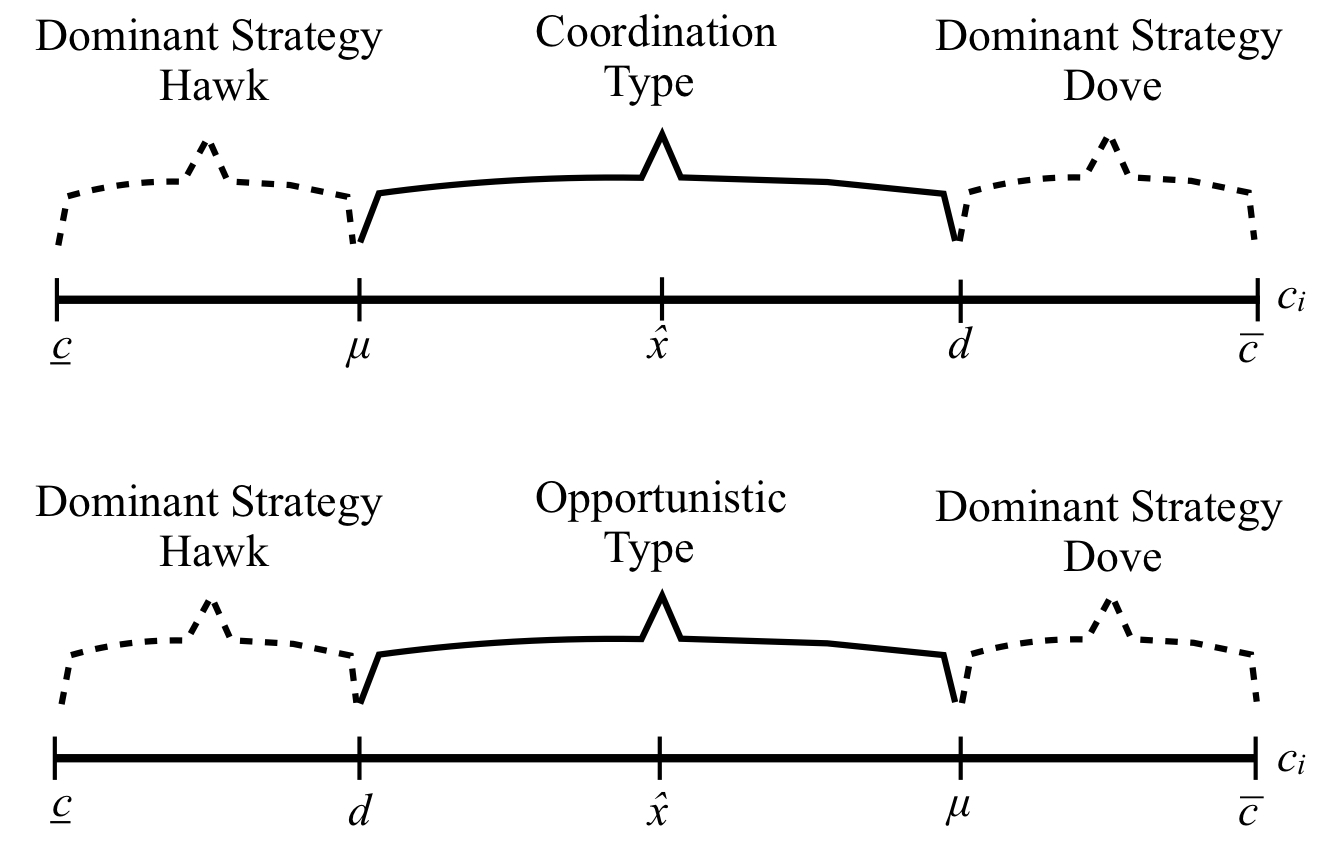
\includegraphics[scale=0.22]{figure1.jpg}
	\caption{Types under strategic complements (top) and substitutes (bottom)}
	\label{fig:1}
\end{figure}
Notice that the game has strategic complements ---the players are coordination types unless they are dominant strategy types--- if $d>\mu$; and the game has strategic substitutes ---the players are opportunistic types unless they are dominant strategy types--- if $\mu> d$. \par
Since player $i$'s expected net payoff from playing $H$ instead of $D$ is monotone in $c_i$, all Bayesian Nash equilibrium (BNE) must be in a cutoff strategy, in which player $i$ has a cutoff point $x_i \in [\underline{c}, \bar{c}]$, where he plays $H$ if and only if $c_i \leq x_i$ (see Figure 1). Specifically, player $i$'s best response to player $j$'s cutoff $x_j$ is the cutoff
\begin{equation}
    x_i=\Gamma(x_j)\equiv \mu+(d-\mu)F(x_j),
\end{equation}
\noindent where the function $\Gamma(\cdot)$ is the best response function for cutoff strategies, and $F(x_j)$ is the probability that player $j$ plays $H$. Lemma 1 states Baliga and Sj\"ostr\"om's (2012 [B]) result for the simultaneous-move conflict games.
\newtheorem{lem}{Lemma}
\begin{lem}
In the unique Bayesian Nash equilibrium (BNE), the probability that player $i$ plays $H$ is $F(\hat{x})$, where $\hat{x}$ is the unique fixed point of $\Gamma(x)$  $ \in [\underline{c}, \bar{c}]$, in equation (1).
\end{lem}\par
Even if player $i$ is not intrinsically hawkish (i.e., non-dominant strategy hawk, $c_i >\mu$), he ends up being hawkish due to the fear of dominant strategy hawks. This reasoning causes spirals of fear (iterated deletion of dominated strategies), which lead to the unique BNE where player $i \in \{A,B\}$ uses the cutoff strategy where he plays $H$ if $c_i \leq \hat{x}$. This is what Baliga and Sj\"ostr\"om (2012 [A]) called ``the Hobbesian trap.''\footnote{Notice that $DD$ Pareto dominates $HH$. But Hobbes singled out $HH$, ``war of every man against every man'', as the more likely outcome in a ``state of nature''. In fact, Hobbes gave a striking argument in favor of this outcome, namely, that there may be some types who actually desire conflict, and this causes everyone to be aggressive in self-defense.}\par
Before we present the extended conflict game with a pre-commitment stage, we set the stage by describing the perfect Bayesian equilibrium (PBE) of the sequential-move conflict game. 

\subsection{The Sequential-Move Conflict Game }
We examine the sequential-move conflict games where player $A$ is the first mover and player $B$ is the second mover. When the game has strategic complements ($d>\mu$), if the first-mover player $A$ plays $D$, then the second-mover player $B$ will play $D$ unless player $B$ is a dominant strategy hawk. That is, if player $A$ plays $D$ first, then player $B$ will become more likely to play $D$, compared to the simultaneous-move game. To see this, player $B$'s probability of playing $D$ is $1-F(\mu)$ in the sequential-move game, whereas it is $1-F(\hat{x})$ in the simultaneous-move game. Hence, it is intuitive that the cutoff point for the first-mover player $A$ to play $H$ in the sequential-move game, labelled as $\bar{x}$, will be smaller than the cutoff point in the simultaneous-move game, $\hat{x}$.\par
Now I formally construct a unique perfect Bayesian equilibrium in the sequential-move game where player $A$ is the first mover, and player $B$ is the second mover.\footnote{Since players $A$ and $B$ are symmetric, the results are symmetric as well if player $B$ moves first.} \par
Consider the conflict game of strategic complements, (i.e., $d>\mu$). Suppose that player $A$, the first mover, uses a cutoff strategy, $\sigma_A(c_A)=H$ if $c_A \leq x$. The strategy of player $B$, the second mover, is $\sigma_B(c_B; a_A)$, where $c_B \in [\underline{c}, \bar{c}]$ and $a_A \in \{H,D\}$, such as $\sigma_B(c_B; H)=H$ if $c_B \leq d$, $\sigma_B(c_B; H)=D$ if $c_B > d$, $\sigma_B(c_B; D)=D$ if $c_B \geq \mu$, and $\sigma_B(c_B; D)=H$ if $c_B < \mu$. Given player $B$'s strategy, player $A$ plays $H$ if the expected payoff of playing $H$ is greater than the expected payoff of playing $D$. That is, player $A$ plays $H$ if $c_A \leq dF(\mu)+\mu(1-F(d))$. Denote $\bar{x}=dF(\mu)+\mu(1-F(d))$. Player $B$'s posterior beliefs are $\rho_B(c_A\leq \bar{x} |H)=1$ and $\rho_B(c_A \leq \bar{x} |D)=0$. Note that $\mu < \bar{x} < d$. \par
%Now consider the conflict game of strategic substitutes, (i.e., $\mu >d$). Suppose that player $A$, the first mover, uses a cutoff strategy, $\sigma_A(c_A)=H$ if $c_A \leq x$. The strategy of player $B$, the second mover, is $\sigma_B(c_B; a_A)$, where $c_B \in [\underline{c}, \bar{c}]$ and $a_A \in \{H,D\}$, such as $\sigma_B(c_B; H)=H$ if $c_B < d$, $\sigma_B(c_B; H)=D$ if $c_B \geq d$, $\sigma_B(c_B; D)=D$ if $c_B > \mu$, and $\sigma_B(c_B; D)=H$ if $c_B \leq \mu$. Given player $B$'s strategy, player $A$ plays $H$ if $c_A \leq \bar{x}$. Player $B$'s posterior beliefs are $\rho_B(c_A\leq \bar{x} |H)=1$ and $\rho_B(c_A \leq \bar{x} |D)=0$.\par
The results are summarized in Lemma 2.
\begin{lem}
There exists a unique perfect Bayesian equilibrium where the first mover uses the cutoff strategy, $\sigma_i(c_i)=H$ if $c_i\leq \bar{x} \equiv dF(\mu)+\mu(1-F(d))$.  In the PBE, $\bar{x}<\hat{x}$ when the game has strategic complements.\footnote{$\hat{x}<\bar{x}$ when the game has strategic substitutes.}
\end{lem}\par
\begin{figure}[t]
\centering
	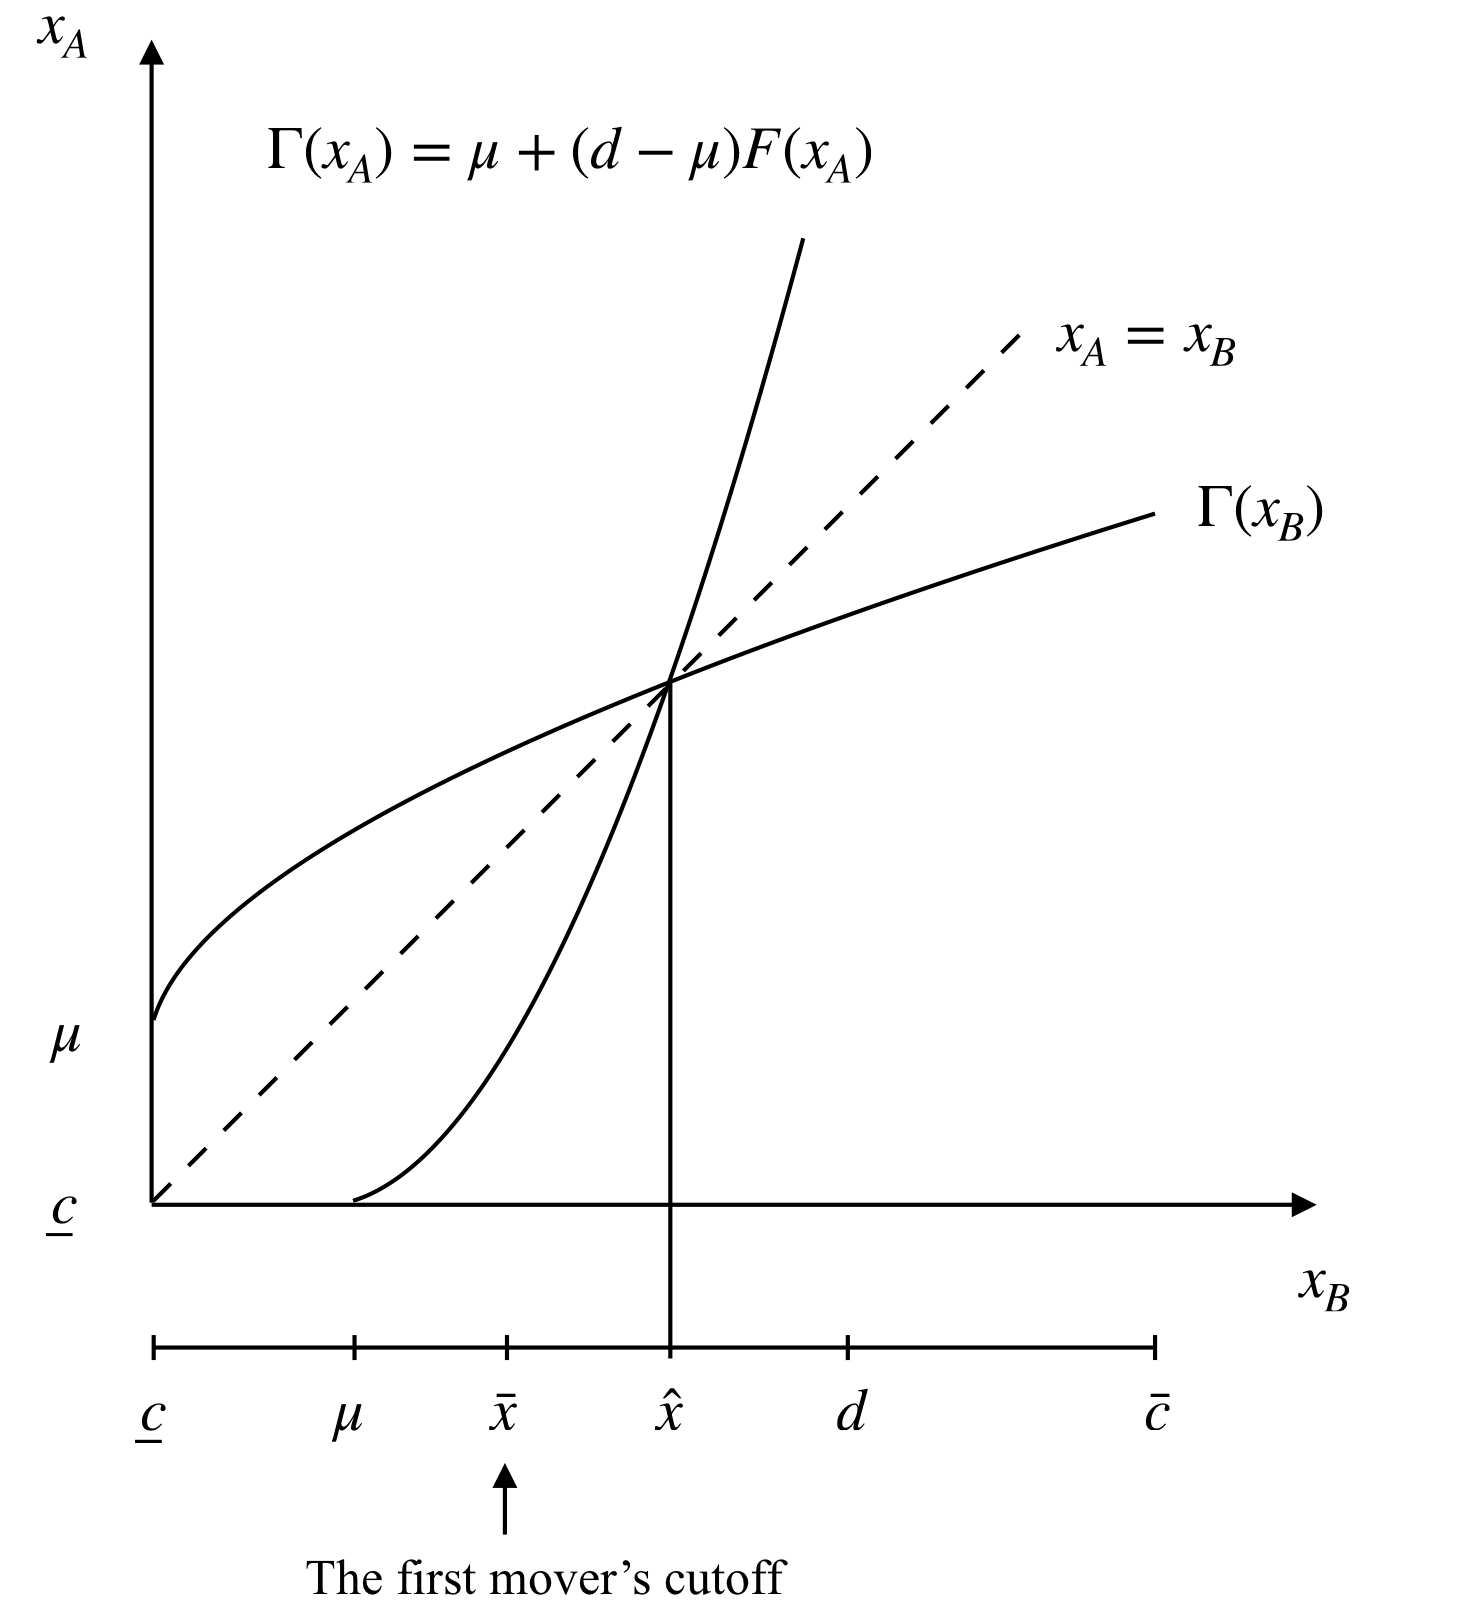
\includegraphics[scale=0.19]{fig2.jpg}
	\caption{The equilibrium cutoffs in the simultaneous-move game (top), and in the sequential-move game (bottom) with strategic complements}
\end{figure}
Note that $\bar{x}<\hat{x}$ if the game has strategic complements\footnote{$\bar{x}>\hat{x}$ if the game has strategic substitutes.} To see this, recall $\hat{x}=dF(\hat{x})+\mu(1-F(\hat{x}))$ and $\bar{x}=dF(\mu)+\mu(1-F(d))$. Since $\mu<\hat{x}<d$ if the game has strategic complements, $F(\mu)<F(\hat{x})$ and $1-F(d)<1-F(\hat{x})$. Hence, $\bar{x}<\hat{x}$.\footnote{Since $d<\hat{x}<\mu$ if the game has strategic substitutes, $F(\mu)>F(\hat{x})$ and $1-F(d)>1-F(\hat{x})$. Hence, $\bar{x}>\hat{x}$.}\par


%Note that $\bar{x}<\hat{x}$ if the game has strategic complements, and $\bar{x}>\hat{x}$ if the game has strategic substitutes. To see this, recall $\hat{x}=dF(\hat{x})+\mu(1-F(\hat{x}))$ and $\bar{x}=dF(\mu)+\mu(1-F(d))$. Since $\mu<\hat{x}<d$ if the game has strategic complements, $F(\mu)<F(\hat{x})$ and $1-F(d)<1-F(\hat{x})$. Hence, $\bar{x}<\hat{x}$. Since $d<\hat{x}<\mu$ if the game has strategic substitutes, $F(\mu)>F(\hat{x})$ and $1-F(d)>1-F(\hat{x})$. Hence, $\bar{x}>\hat{x}$.\par
%When the game has strategic substitutes (i.e., $d<\mu$), if the first-mover player $A$ plays $D$, then the second-mover player $B$ will play $H$ unless player $B$ is a dominant strategy dove. That is, if player $A$ plays $D$ first, then player $B$ will be less likely to play $D$, compared to the simultaneous-move game. To see this, the probability of playing $D$ is $1-F(\mu)$ in the sequential-move game, whereas it is $1-F(\hat{x})$ in the simultaneous-move game. Hence, it is intuitive that the cutoff point to play $H$ for the first-mover player $A$ in the sequential-move game, $\bar{x}$, is larger than the cutoff point in the simultaneous-move game, $\hat{x}$.\par
Lastly, it is important to note that the players' reasoning to reach to the equilibrium in the sequential-move game differs from that in the simultaneous-move game. In the simultaneous-move game (with strategic complements), the players' mutual fear of dominant strategy hawks (mutual beliefs that the opponent can be a dominant strategy hawk) causes a subset of coordination types to play $H$, (i.e., $\sigma_i(c_i)=H$ if $c_i \leq \hat{x}$). In the sequential-move game, however, the mutual fear is removed due to the fact that the second mover's action will simply depend on the observed action taken by the first mover;  and this in turn causes the first mover less likely to play $H$, compared to the simultaneous-move game. 

\subsection{The Extended Conflict Game with a Pre-commitment Stage}
Here, we present the extended conflict game. The question is whether a dovish player will decide to commit to an early dovish action in the presence of uncertainty about the opponent's type. To isolate the pure logic for the question of which action appears first when the players are allowed to commit to an action in a preplay stage, we extend the conflict game with a pre-commitment stage. That is, in a preplay stage, the players simultaneously decide whether to move early or late. If a player decides to move early, he can do so only by selecting an action to which it is then committed. A player who chooses to move late does not make such action commitment.\footnote{Hamilton and Slutsky (1990) first lay out this rule of endogenous timing in the form of the extended game with action commitment in a duopoly game under complete information.} Formally, the game proceeds as follows.\par
\begin{itemize}\itemsep-2pt 
\item \textbf{Stage 0:} Player $i \in \{A,B\}$ observes her type $c_i$, but not the other player's type $c_j$ where $j\neq i$.
\item \textbf{Stage 1:} Players $A$ and $B$ simultaneously decide $(t_{i}=1; H)$, $(t_{i}=1; D)$, or $t_i=2$, for $i=\{A,B\}$. 
\item \textbf{Stage 2:} The conflict game is played according to the move structure determined in Stage 1.
\end{itemize}\par
\begin{figure}[t]
\centering
	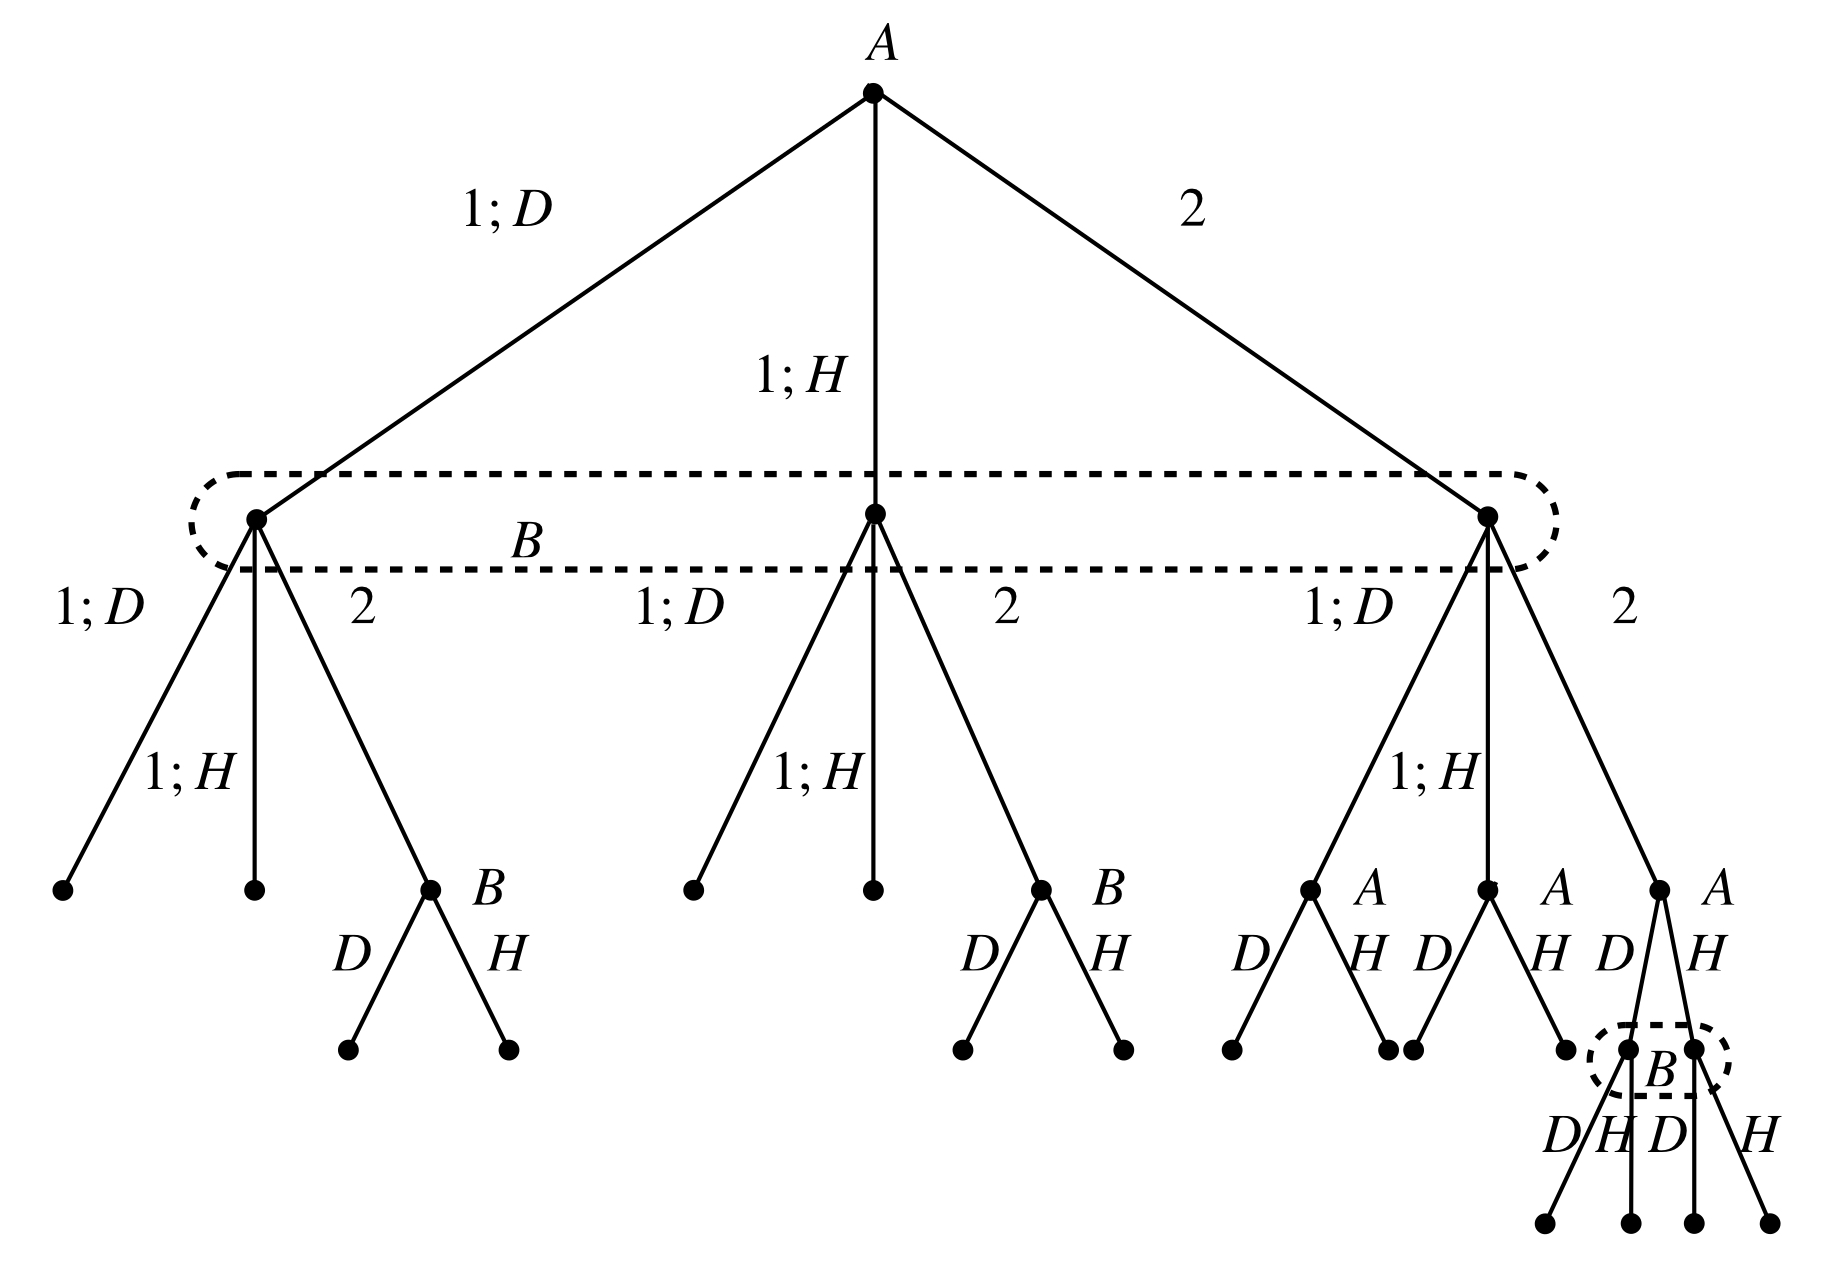
\includegraphics[scale=0.18]{fig3.jpg}
	\caption{The extended conflict game with action commitment}
\end{figure}\par
The extensive form of the extended conflict game with action commitment is described in Figure 3.\par 
If they play the simultaneous-move game late in the second period, it indicates that they both declined to commit to playing an early action. Thus, they will update the prior beliefs before they choose an action in the second period. A sequential-move game will be played if one player commits to an early action in the first period, and the other player chooses to play late in the second period. Note that the second mover will observe the action played by the first mover before he chooses an action in the second period; and a player who commits to an early action must decide to do so based on the prior belief. Therefore, a player will decide to move early and to commit to an early action if and only if the ex-ante (preplay) expected payoff from playing an early action, either $H$ or $D$, is greater than the expected payoff from waiting. \par 
Note that there exists a pooling equilibrium where every type $c_i \in [\underline{c}, \bar{c}]$ is pooling to the same period. Then, the simultaneous-move game will be played, and simply Lemma 1 is invoked for the pooling equilibrium. \par 
Moreover, and most importantly, we examine whether there exists a separating equilibrium, where a subset of types commits to an early dovish action (i.e., $t_i=1;D$) while other types wait (i.e., $t_i=2$). By Lemma 2, we conjecture that there exists a separating equilibrium strategy that a player whose type is greater than $\bar{x}$ chooses to move early with action commitment to $D$.\footnote{Note that the extended game can proceed as follows: In Stage 1, if a player decides to commit to an early action, either $H$ or $D$, he must do so by declaring ``If I move first, I will commit to $D$ (or $H$).'' Indeed, by Lemma 2, the first-mover player will play $D$ if his type is $c_i > \bar{x}$, and $H$ if otherwise.} The results are summarized in Proposition 1.\par
\newtheorem{prop}{Proposition}
\begin{prop}
In the extended conflict game of strategic complements, there exist a unique separating equilibrium, where the players' strategies are: $t_{i}(c_i)=1; D$ for $c_i >\bar{x}$, and $t_{i}(c_i)=2$ for $c_{i} \leq \bar{x}$.\footnote{It is straightforward that a separating equilibrium does not exist in the extended conflict game of strategic substitutes because players are opportunistic when the game has strategic substitutes unless they are dominant strategy types.}
\end{prop}\par
\begin{proof}
See Appendix.
\end{proof}\par
To illustrate, with strategic complements a player only wants to move early if he plans to choose $D$. Thus, the dovish players (high-cost types) move early and commits to $D$. Dominant strategy hawks of course wait and choose $H$ as late as possible. Finally, the in-between types have a \textit{wait-and-see} attitude: they are unwilling to commit too early, but if the opponent commits to $D$, they will respond with $D$. \par 
Consequently, the likelihood of the peaceful outcome $DD$ increases, compared to the simultaneous-move game. Specifically, the likelihood of the peaceful outcome in the simultaneous-move game is $(1-F(\hat{x}))(1-F(\hat{x}))$, while it is $(1-F(\bar{x}))(1-F(\mu))$ in the extended conflict game with action commitment. To see this, the probability that a player moves first and plays $D$ is ($1-F(\bar{x})$), which is equal to the likelihood that the player's type is drawn from $(\bar{x}, \bar{c}]$; and the probability that the other player plays $D$, either in the first period or in the second period, is ($1-F(\mu)$), which is equal to the likelihood that the player's type is drawn from $[\mu, \bar{c}]$.\par
\newtheorem{corol}{Corollary}
\begin{corol}
In the extended conflict game of strategic complements with action commitment, the likelihood of the peaceful outcome $DD$ is greater than that in the simultaneous-move game. 
\end{corol}\par

\subsection{The Conflict Game in the Lab}
\label{sec:model}
For our lab experiment, we convert the conflict game in Table 1 as the following payoff matrix:
\begin{equation}
\begin{pmatrix}
x_i & \mu+x_i \\
k-d & k 
\label{t:payoff}
\end{pmatrix},
\end{equation}
where $k=100$, $\mu=10$, and $d=95$.\footnote{Only the case of strategic complements is considered in our lab experiment.} When player $i \in \{A,B\}$ plays $H$, he receives $x_i$, which corresponds to his type, $c_i$. Note that $x_i$ is independently drawn from a uniform distribution $F\in [0,k]$. That is, some players are revealed to be more hawkish and thus reap more benefit from action $H$, and some are revealed to be less hawkish and see a lower return to playing $H$. If both players choose the dovish action $D$, then the payoff to each player is a constant $k$. If player $i$ plays $D$, while player $j\neq i$ plays $H$, then the payoff to player $i$ is $k-d>0$, where $d$ can be considered a cost of a dovish action when the opponent is aggressive. On the other hand, if player $i$ plays $H$ and player $j\neq i$ plays $D$, then the payoff to player $i$ is $\mu+x_i$, where $\mu$ can be viewed as a benefit of an aggressive action when the opponent is dovish.  \par
The unique cutoff point of the BNE in the simultaneous-move game (one-shot conflict game, hereafter CGO) is
\begin{equation}
\hat{x}_{_{CGO}}:= k-d + (d-\mu) F(\hat{x}_{_{CGO}}). \label{eq:cgo}
\end{equation}

\noindent Given that $F(\cdot)$ follows a uniform distribution in the space $[0,k]$, the cutoff point of a CGO can be rewritten as 
\begin{equation}
\hat{x}_{_{CGO}}= \frac{k\cdot (k-d)}{k-d+\mu}=33. \label{eq:cgosol}
\end{equation}\par
In the sequential-move conflict game (hereafter CGS), the equilibrium cutoff point for the first mover is 
\begin{equation}
\sigma_i(x_i)=D \quad \text{if} \ \ x_i\leq \hat{x}_{_{CGS}}:= k-\mu=90. 
\end{equation}\par
Next, the extended conflict game with action commitment (hereafter CGE) proceeds as follows:
\begin{itemize}\itemsep-2pt
\item \textbf{Stage 0:} Each player $i$ selects a cutoff strategy, indicating a set of values where $\sigma_i(x_i)=H$, and then observes own type $x_i$, but not the other player's type $x_j$ where $j\neq i$.

\item \textbf{Stage 1:} Both players simultaneously select the period in which to play the game $t=1,2$. 

\item \textbf{Stage 2:} The conflict game is played by the move structure determined in Stage 1. The commitment to the cutoff strategy is not binding for player $i$ if and only if $t_i=2$ and $t_j=1$.\footnote{In theory, the players' cutoff strategy is not binding if both players choose to wait (i.e., $t_i=2$ for $i \in \{A,B\}$). Here, we make them binding because we restrict our attention to the players' cutoff strategy in our experiment.} 
\end{itemize}\par

Recall that in theory the CGE has two equilibria, pooling and separating. If every type selects the same time period (e.g. $t=2$), then the environment resembles the CGO and the equilibrium follows the cutoff strategy specified in (3): $\hat{x}_{_{CGE}}=\hat{x}_{_{CGO}}=33$ (the pooling equilibrium). Alternatively, if a player expects the game to progress sequentially, then the equilibrium cutoff point will be $\hat{x}_{_{CGE}}=\hat{x}_{_{CGS}}=90$, where type $x\leq \hat{x}_{_{CGS}}\equiv 90$ will select $t=1$ and commit to $D$, while type $x>\hat{x}_{_{CGS}}$ will wait to play at $t=2$ (the separating equilibrium). \\

\noindent \textbf{Hypothesis 1}
\textit{In the CGO, subjects play at or above the cutoff strategy $\hat{x}_{_{CGO}}=33$.}\\

We reconcile the theoretical solution of the CGO with experimental evidence for our first prediction. In the laboratory, subjects play $D$ more often than predicted by the Nash Equilibrium (NE). \\

\noindent \textbf{Hypothesis 2}
\textit{The cutoff strategy in the CGS is higher compared to the cutoff strategy in the CGO.}\\

Note that the equilibrium predictions $\hat{x}_{_{CGS}}=90$ and $\hat{x}_{_{CGO}}=33$ are far apart. This allows us to observe meaningful differences even when players chose cutoff values greater than the NE described in Prediction 1. The gain in expected payoff is equal to $d\times \left( F(\hat{x}_{_{CGS}})-F(\hat{x}_{_{CGO}}) \right)=95\times( 90-33)/100=50$ points or 137 percent. \\

\noindent \textbf{Hypothesis 3A} \textit{In the CGE, a player will behave as in the CGO. }\\
\noindent \textbf{Hypothesis 3B} \textit{In the CGE, a player will behave as in the CGS.}\\

As the CGE can lead to multiple equilibria, we are uncertain about the type of equilibrium that would prevail in our experiment. The two conflicting Predictions, 3A and 3B, reflect the pooling equilibrium and the separating equilibrium, respectively. Our experiment is designed to test which type of equilibrium, if any, will prevail. \\

\noindent \textbf{Hypothesis 4}
\textit{The frequency of a $DD$ outcome in the CGS is greater than the frequency of a $DD$ outcome in the CGO. In the CGE, the frequency of $DD$ is no smaller than in the CGO.}

\\


The coordination required to achieve the $DD$ outcome should be easier to achieve in a sequential game. Therefore, the frequency of $DD$ should be higher in the CGS relative to the CGO. The CGE can lead to two outcomes, both of which depend on the selected order of play and the type of equilibrium when the players choose the cutoff. No matter what type of equilibrium prevails, we expect that the frequency of $DD$ in the CGE will be no lower than that in the CGO.   \\

\noindent \textbf{Hypothesis 5}
\textit{There is no gender difference in strategy choices across the three treatments.}\\

Gender differences in cooperative behavior and social dilemma environments have been studied using games such as Prisoners Dilemma (PD) and Stag hunt. Literature from psychology suggests that women are more cooperative
than men. Fehr et al show that women tend to be more egalitarian. 

However, in PD game in particular, no consistent gender difference is observed. 

The PD game muddles up motivations of each gender and this explains the lack of a result.

Simpson (2003) and Kuwabara (2005) have argued that gender does matter because men and women have different motivations. Males are motivated by greed, and will defect from cooperation because of greed, as well as free-ride on the cooperation of others. Females, on the other hand, are motivated by fear and will defect
to avoid being exploited. In other words, they fear the greed of their partner. 
This can also be argued is a fear of being out of control. By choosing H, women maintain control over their destiny (payoff). Also, if women fear men are less egalitarian, more accepting of inequality, and
more competitive and more desirous of being first, better to choose $H$. Choosing $D$ leaves women at the mercy of their counterparty (recall that we work with gender balance sessions). In PD game both greed and fear
are at play leading to both genders playing the game in a similar fashion.

In our CGO treatment, both players move simultaneously. The fear/greed arguments would suggest that men will want to play $H$ out of a desire to exploit cooperative partners. Women will play $H$ out of a desire not to be exploited and a fear their partners will be greedy and play $H$.

The shift in the cutoff in the CGS game can be explained by the reduced risk. In CGS, the sequence of play is exogenously determined. So there is a 50 percentage chance of moving second. Men will want to play $H$ out of a desire to exploit cooperative partners, but less than in CGO since second movers can alter choice to reflect first movers’ decisions. Greed will make some men willing to choose $D$ if they are the second mover. Women will still be more likely to play $H$ out of a desire not to be exploited and a fear their partners will be greedy and play $H$, again less so since second movers can change decisions.  Thus, men's cutoff shift right out of greed. They can choose $D$ since if they end up as first mover, they can rely on the greed of fellow men and the egalitarianism of women second movers to choose $D$. Women can shift cutoff right, since the probability of exploitation is less than in CGO game. 

Finally, in the CGE game, there is a uncertainty about the type of encounter a player will face. Fear from either men or women can trigger a cutoff choice similar to the CGO game, which is reinforced with the lack of coordination between parties. The greed for men is not enough to sustain a $DD$ outcome since it is not guaranteed that another player will wait and see in the second period, and rather reap off the gains from playing $H$ when another commits to $D$.



\newpage

\section*{Appendix: Proofs}

%The ex-ante expected payoffs in the pooling equilibrium are, 
%\begin{equation*}
   %\pi^p_{i} = 
   %\begin{cases}
    %\mu (1-F(\hat{x}))-c_{i}, &  \text{if} \  c_{i}\leq %\hat{x};\\
    %-F(\hat{x})d, & \text{otherwise}.
   %\end{cases}
%\end{equation*}\par
We will construct a unique separating equilibrium where a subset of types ($c_i > \bar{x}$) commits to an early dovish action (i.e., $t_i=1;D$), while other types ($c_i \leq \bar{x}$) wait (i.e., $t_i=2$).\par
(i) Consider the following candidate separating-equilibrium strategy for player $i \in \{A,B\}$:
\begin{align}
 t_i(c_i)=
 \begin{cases} 1; H, \mbox{ if } c_i \leq \bar{x}, \\
 2, \mbox{ if } c_i > \bar{x}.
 \end{cases}
\end{align}\par
Suppose that player $i$'s type is $c_i > \bar{x}$, and that he chooses $t_i(c_i)=2$ by following the strategy (6). Since the probability that player $j \neq i$ chooses $t_j=2$ is $1-F(\bar{x})$, the late simultaneous-move game will be played with probability $1-F(\bar{x})$, and the sequential-move game where player $i$ is the second mover will be played with probability $F(\bar{x})$.\par
If $t_i(c_i)=2$ for $i \in \{A,B\}$, then each player will update beliefs such that $c_j > \bar{x}$. In this case, the preplay timing strategy completely eliminates the probability that the opponent is a dominant strategy hawk, thus there is no incentive to play $H$ for both players.\footnote{See Baliga and Sj\"ostr\"om (2004, 2012 [A]) for the truncated simultaneous-move game.} \par 
If $t_j(c_j)=1; H$, then the second-mover player $i$ will play $H$ as well unless player $i$ is a dominant strategy dove. Hence, player $i$'s ex-ante expected payoff from $t_i(c_i)=2$ is
\begin{equation}
\pi_i(t_i=2)=F(\bar{x})\cdot (-c_i)+(1-F(\bar{x})) \cdot 0=-c_iF(\bar{x}),
\end{equation}
if player $i$ is a dovish-coordination type (i.e., $c_i \in (\bar{x},d$]); and
\begin{equation}
\pi_i(t_i=2)=F(\bar{x})\cdot (-d)+(1-F(\bar{x})) \cdot 0=-dF(\bar{x}),
\end{equation}
if player $i$ is a dominant strategy dove (i.e., $c_i > d$).\par
Now, suppose that player $i$'s type is $c_i \leq \bar{x}$, and that he chooses $t_i(c_i)=1; H$ by following the strategy (6). Then, the early simultaneous-move game will be played with probability $F(\bar{x})$; and the sequential-move game where player $i$ is the first mover will be played with probability $1-F(\bar{x})$. \par 
If $t_i(c_i)=1; H$ for $i \in \{A,B\}$, it becomes the early simultaneous-move game where both play $H$. If $t_j(c_j)=2$, then the second-mover player $j$ will play $H$ with probability $F(d)-F(\bar{x})$, and play $D$ with probability $1-F(d)$. Hence, player $i$'s ex-ante expected payoff from $t_i(c_i)=1; H$ is
\begin{align}
\pi_i(t_i=1; H)&=F(\bar{x})\cdot (-c_i)+(1-F(\bar{x})) [-c_i (F(d)-F(\bar{x})) +(\mu-c_i)(1-F(d))]\\
&=-c_iF(\bar{x})+(1-F(\bar{x}))[-c_i(1-F(\bar{x}))+\mu(1-F(d))] \notag \\
&=-c_iF(\bar{x})+(1-F(\bar{x}))[\mu-c_i+c_iF(\bar{x})-\mu F(d)]. \notag
\end{align}\par
To see whether the strategy (6) is an equilibrium strategy, we check whether a hawkish player $i$ whose type is $c_i \leq \bar{x}$ has an incentive to deviate to the second period. The ex-ante expected payoff from deviation to the second period is
\begin{equation}
\pi_i(t_i=2)=F(\bar{x}) \cdot (-c_i) +(1-F(\bar{x})) \cdot 0=-c_iF(\bar{x}) \notag
\end{equation}
for a hawkish-coordination type (i.e., $ c_i \in (\mu, \bar{x}$]); and
\begin{equation}
\pi_i(t_i=2)=F(\bar{x}) \cdot (-c_i) +(1-F(\bar{x})) \cdot (\mu-c_i) \notag
\end{equation}
for a dominant strategy hawk (i.e., $c_i \leq \mu$). \par 
It is straightforward to see that the payoffs from deviation to the second period exceed the payoffs from $t_i(c_i)=1; H$. Specifically, for a hawkish-coordination type ($\mu< c_i \leq \bar{x}$), 
\begin{align*}
\pi_i(t_i=2)&=-c_iF(\bar{x})>\\
&\pi_i(t_i=1; H)=F(\bar{x})\cdot (-c_i)+(1-F(\bar{x})) [-c_i (F(d)-F(\bar{x})) +(\mu-c_i)(1-F(d))],
\end{align*}
since $F(d)-F(\bar{x})>0$, $1-F(d)>0$, $-c_i <0$, and $\mu-c_i<0$. For a dominant strategy hawk type ($c_i \leq \mu$),
\begin{align*}
\pi_i(t_i=2)=F(\bar{x})& \cdot (-c_i) +(1-F(\bar{x})) \cdot (\mu-c_i)>\\
&\pi_i(t_i=1; H)=-c_iF(\bar{x})+(1-F(\bar{x}))[-c_i(1-F(\bar{x}))+\mu(1-F(d))].
\end{align*}
To prove this, suppose that $\mu-c_i < \mu(1-F(d))-c_i(1-F(\bar{x}))$, which indicates that $\mu \frac{F(d)}{F(\bar{x})} < c_i$. However, this is contradiction because player $i$ is a dominant strategy hawk ($c_i \leq \mu$) and  $\mu \frac{F(d)}{F(\bar{x})}>\mu$. Hence, the strategy (6) cannot be an equilibrium strategy.\par
(ii) Consider the following candidate separating-equilibrium strategy for player $i \in \{A,B\}$:
\begin{align}
 t_i(c_i)=
 \begin{cases} 1; D, \mbox{ if } c_i > \bar{x}, \\
 2, \mbox{ if } c_i \leq \bar{x},
 \end{cases}
\end{align}
which is the reverse of (6). \par 
Suppose that player $i$'s type is $c_i \leq \bar{x}$, and that he chooses $t_i(c_i)=2$ by following the strategy (10). Since the probability that player $j \neq i$ chooses $t_j=2$ is $F(\bar{x})$, the late simultaneous-move game will be played with probability $F(\bar{x})$, and the sequential-move game where player $i$ is the second mover will be played with probability $1-F(\bar{x})$.\par
If $t_i(c_i)=2$ for $i \in \{A,B\}$, then each player will update beliefs such that $c_j \leq \bar{x}$, where $\bar{x}<d$. In this case, the preplay timing choice completely eliminates the probability that the opponent chooses $D$, and there exists a unique BNE where all types $c_i \in [\underline{c}, \bar{x}$] play $H$ with probability one. \par
If $t_j(c_j)=1; D$, then the second-mover player $i$ will play $D$ unless he is a dominant strategy hawk. Hence, player $i$'s ex-ante expected payoff from $t_i(c_i)=2$ is
\begin{equation}
\pi_i(t_i=2)=F(\bar{x})\cdot (-c_i)+(1-F(\bar{x})) \cdot 0=-c_iF(\bar{x}),
\end{equation}
for a hawkish-coordination type (i.e., $c_i \in (\mu, \bar{x}]$); and
\begin{equation}
\pi_i(t_i=2)=F(\bar{x})\cdot (-c_i)+(1-F(\bar{x})) (\mu-c_i)=\mu(1-F(\bar{x}))-c_i,
\end{equation}
for a dominant strategy hawk (i.e., $c_i \leq \mu$).\par
%Note that, if player $i$ is a hawkish type, (i.e., $c_i \leq \bar{x}$), player $i$ will always have an incentive to switch to the second period by following the timing strategy (6). To see this, for a hawkish-coordination type, (i.e., $\mu<c_i \leq \bar{x}$), the ex-ante expected payoff of announcing the second period (the payoff expression (7)) is greater than the ex-ante expected payoff of announcing the first period (the payoff expression (5)). For a dominant strategy hawk, the ex-ante expected payoff (8) is greater than the ex-ante expected payoff (5) as well. To see this, suppose that 
%\begin{equation}
%c_iF(\bar{x})-\mu F(d)>0, \notag
%\end{equation}
%which yields $c_i > \mu \frac{F(d)}{F(\bar{x})}$ ($> \mu$). However, this is contradiction since player $i$ is a dominant strategy hawk, (i.e., $c_i \leq \mu$). Hence, it must be that $c_iF(\bar{x})-\mu F(d)<0$, and thereby the ex-ante expected payoff (8) is greater than the ex-ante expected payoff (5). Therefore, the timing strategy (2) cannot be the equilibrium strategy for hawkish types ($c_i \leq \bar{x}$).\par
%Next, we need to check if a dovish player whose type is $c_i > \bar{x}$ will follow the timing strategy (6) as well. Let us calculate player $i$'s ex-ante expected payoff of announcing the first period:
Next, suppose that player $i$'s type is $c_i > \bar{x}$, and that he chooses $t_i(c_i)=1; D$ by following the strategy (10). Then, the early simultaneous-move game will be played with probability $1-F(\bar{x})$; and the sequential-move game where player $i$ is the first mover will be played with probability $F(\bar{x})$. Hence, player $i$'s ex-ante expected payoff from $t_i(c_i)=1; D$ is
\begin{align}
\pi_i(t_i=1; D)&=F(\bar{x})[(F(\bar{x})-F(\mu)) \cdot 0 +F(\mu) (-d)] +(1-F(\bar{x})) \cdot 0\\
&=-dF(\bar{x})F(\mu).\notag
\end{align}\par
To see whether that the strategy (10) is an equilibrium strategy, we check whether a dovish player $i$ whose type is $c_i > \bar{x}$ has an incentive to deviate to the second period. The ex-ante expected payoff from deviation to the second period is
\begin{equation}
\pi_i(t_i=2)=F(\bar{x}) \cdot (-c_i) +(1-F(\bar{x})) \cdot 0=-c_iF(\bar{x}) \notag
\end{equation}
for a dovish-coordination type (i.e., $c_i \in (\bar{x},d]$); and
\begin{equation}
\pi_i(t_i=2)=F(\bar{x}) \cdot (-d) +(1-F(\bar{x})) \cdot 0=-dF(\bar{x}) \notag
\end{equation}
for a dominant strategy dove (i.e., $c_i > d$). \par
It is straightforward to see that there is no incentive for a dovish player whose type is $c_i > \bar{x}$ to deviate to the second period.  To see this, for a dovish-coordination type ($\bar{x}<c_i \leq d$), suppose that 
\begin{align*}
\pi_i(t_i=2)=-c_iF(\bar{x})> \pi_i(t_i=1; D)=-dF(\bar{x})F(\mu),
\end{align*}
which yields $c_i < dF(\mu)$. However, this is contradiction because player $i$'s type is $\bar{x}=dF(\mu)+\mu(1-F(d)) < c_i \leq d$. Hence, $\pi_i(t_i=2)=-c_iF(\bar{x})< \pi_i(t_i=1; D)=-dF(\bar{x})F(\mu)$; and a dovish-coordination type does not have any incentive to deviate to the second period.\par 
For a dominant strategy dove ($c_i>d)$, it is straight forward that $\pi_i(t_i=2)=-dF(\bar{x})< \pi_i(t_i=1; D)=-dF(\bar{x})F(\mu)$; hence, a dominant strategy dove does not have any incentive to deviate to the second period. \par 
Next, we need to check whether a hawkish player whose type is $c_i \leq \bar{x}$ has an incentive to deviate to play $H$ in the first period. The ex-ante expected payoff from deviation is
\begin{equation}
\pi_i(t_i=1;H)=F(\bar{x})\cdot(-c_i)+(1-F(\bar{x}))\cdot (\mu-c_i) = \mu(1-F(\bar{x})) -c_i. \notag
\end{equation}
For a hawkish-coordination type (i.e., $c_i \in (\mu, \bar{x}]$), the ex-ante payoff from $t_i(c_i)=2$ is $\pi_i(t_i=2)=-c_iF(\bar{x})$. Suppose that the ex-ante expected payoff from deviation to the first period exceeds that from $t_i(c_i)=2$. That is,
\begin{equation}
\pi_i(t_i=2)=-c_iF(\bar{x})< \pi_i(t_i=1;H)= \mu(1-F(\bar{x})) -c_i,\notag
\end{equation}
which yields $c_i <\mu$. However, this is contradiction because player $i$'s type is $c_i \in (\mu, \bar{x}]$. Thus, a hawkish-coordination type does not have an incentive to deviate to play $H$ in the first period.\par
For a dominant strategy hawk (i.e., $c_i \leq \mu$), the ex-ante payoff from deviation is equal to that from $t_i(c_i)=2$. That is, 
\begin{equation}
\pi_i(t_i=2)=F(\bar{x})\cdot (-c_i)+(1-F(\bar{x})) (\mu-c_i)=\mu(1-F(\bar{x}))-c_i=\pi_i(t_i=1;H). \notag
\end{equation}
Thus, a dominant strategy hawk does not have an incentive to play $H$ in the first period. Therefore, the separating strategy (10) is an equilibrium strategy. \qed \par
%To see if the ex-ante expected payoff (9) is greater than the ex-ante expected payoff (3), suppose that the payoff (3) is greater than the payoff (9):
%\begin{equation}
%-c_iF(\bar{x})>-dF(\bar{x})F(\mu), \notag
%\end{equation}
%which yields $c_i < dF(\mu)$. However, this is contradiction because player $i$ is a dovish player, (i.e., $c_i > \bar{x}=F(\mu)d+\mu(1-F(d)))$. Hence, it must be that $-c_iF(\bar{x})<-dF(\bar{x})F(\mu)$. Thus, the ex-ante expected payoff (9) is greater than the ex-ante expected payoff (3). In sum, every type $c_i \in [\underline{c}, \bar{c}]$ is better off choosing the timing strategy (6). \par 









%\singlespacing
\setlength\bibsep{0pt}
\bibliographystyle{my-style}
\bibliography{Placeholder}



%\clearpage

%\onehalfspacing

%\section*{Tables} \label{sec:tab}
%\addcontentsline{toc}{section}{Tables}



%\clearpage

%\section*{Figures} \label{sec:fig}
%\addcontentsline{toc}{section}{Figures}

%\begin{figure}[hp]
%  \centering
%  \includegraphics[width=.6\textwidth]{../fig/placeholder.pdf}
%  \caption{Placeholder}
%  \label{fig:placeholder}
%\end{figure}




\clearpage

\section*{References} \label{sec:appendixa}

\noindent
\hangindent 12pt
\textbf{Baliga, Sandeep, and Tomas Sj\"ostr\"om.} 2004. ``Arms Races and Negotiations." \textit{Review of Economic Studies} 71: 351-369.

\noindent
\hangindent 12pt
\textbf{Baliga, Sandeep, and Tomas Sj\"ostr\"om.} 2009. ``Conflict Games with Payoff Uncertainty." Unpublished.

\noindent
\hangindent 12pt
\textbf{Baliga, Sandeep, and Tomas Sj\"ostr\"om.} 2012 [A]. ``The Hobbesian Trap." In \textit{The Oxford Handbook of the Economics of Peace and Conflict}, edited by Michelle R. Garfinkel and Stergios Skaperdas. New York: Oxford University Press.

\noindent
\hangindent 12pt
\textbf{Baliga, Sandeep, and Tomas Sj\"ostr\"om.} 2012 [B]. ``The Strategy of Manipulating Conflict." \textit{American Economic Review} 102 (6): 2897-2922.

\noindent
\hangindent 12pt
\textbf{Hamilton, Jonathan H., and Steven M. Slutsky.} 1990. ``Endogenous Timing in Duopoly Games: Stackelberg or Cournot Equilibria." \textit{Games and Economic Behavior} 2: 29-46.

\noindent
\hangindent 12pt
\textbf{Hobbes, Thomas.} 1651. \textit{Leviathan}. London: Penguin Books.


%\noindent
%\hangindent 12pt
%\textbf{Kimbrough, E.O., Laughren, K. and Sheremeta, R.}, 2017. ``War and conflict in economics: Theories, applications, and recent trends. \textit{Journal of Economic Behavior & Organization}.





\noindent
\hangindent 12pt
\textbf{Schelling, Thomas C.} 1960. \textit{The Strategy of Conflict}. Cambridge: Harvard University Press.

\end{document}

We formally present the separating equilibrium of the extended conflict game with action commitment. After the preplay stage (Stage 1), the players will update beliefs about the opponent's type. Given their posterior beliefs, the players' strategies must be sequentially rational. Formally, player $i$'s strategy in Stage 2 is $\sigma_i$: $C_i \times \{(1,1), (1,2), (2,1) \times a_j, (2,2)\} \rightarrow a_i \in\{H,D\}$, where $a_j \in \{H,D\}$ is player $j$'s action when player $j$ is the first mover, and $C_i = [\underline{c}, \bar{c}]$ is the type space of player $i$. Likewise, player $j$'s strategy in Stage 2 is $\sigma_j$: $C_j \times \{(1,1), (1,2) \times a_i, (2,1), (2,2)\} \rightarrow a_j \in\{H,D\}$, where $a_i \in \{H,D\}$ is player $i$'s action when player $i$ is the first mover, and $C_j = [\underline{c}, \bar{c}]$ is the type space of player $j$. The posterior beliefs about the opponent's type is $\rho_i(a_j=H|(t_i,t_j))$. Lastly, the players' strategy of timing must be optimal, given the players' subsequent strategies and beliefs.  \par 
The perfect Bayesian equilibrium strategy profiles and beliefs proceed as follows. \par
\begin{itemize}\itemsep-2pt
\item $\sigma_i(c_i,(1,1))=D$, $\sigma_j(c_j,(1,1))=D$, $\rho_i(H|(1,1))=0$, and $\rho_j(H|(1,1))=0$, if $c_i>\bar{x}$ and $c_j>\bar{x}$; 
\item $\sigma_i(c_i,(1,2))=D$, $\sigma_j(c_j,H,(1,2))=H$, $\sigma_j(c_j,D,(1,2))=D$, $\rho_i(H|(1,2))=F(\mu)$, $\rho_j(H|(1,2))=0$, if $c_i>\bar{x}$ and $\mu<c_j\leq \bar{x}$; 
\item $\sigma_i(c_i,(1,2))=D$, $\sigma_j(c_j,H,(1,2))=H$, $\sigma_j(c_j,D,(1,2))=H$, $\rho_i(H|(1,2))=F(\mu)$, $\rho_j(H|(1,2))=0$, if $c_i>\bar{x}$ and $c_j < \mu$;
\item $\sigma_i(c_i,H,(2,1))=H$, $\sigma_i(c_i,D,(2,1))=D$, $\sigma_j(c_j,(2,1))=D$, $\rho_i(H|(2,1))=0$, $\rho_j(H|(2,1))=F(\mu)$, if $\mu \leq c_i \leq \bar{x}$ and $c_j > \bar{x}$; 
\item $\sigma_i(c_i,H,(2,1))=H$, $\sigma_i(c_i,D,(2,1))=H$, $\sigma_j(c_j,(2,1))=D$, $\rho_i(H|(2,1))=0$, $\rho_j(H|(2,1))=F(\mu)$, if $c_i < \mu$ and $c_j > \bar{x}$; and 
\item $\sigma_i(c_i,(2,2))=H$, $\sigma_j(c_j,(2,2))=H$, $\rho_i(H|(2,2))=1$, $\rho_j(H|(2,2))=1$, if $c_i \leq \bar{x}$ and $c_j \leq \bar{x}$. 
\end{itemize}\par 

\subsubsection{Strategic Substitutes}
Now we examine the case in which the game has strategic substitutes, (i.e., $d<\mu$). Consider the following separating strategy for player $i \in \{A,B\}$:
\begin{align}
 t_i(c_i)=
 \begin{cases} 1;H, \mbox{ if } c_i \leq \bar{x}, \\
 2, \mbox{ if } c_i > \bar{x}.
 \end{cases}
\end{align}\par
It is straightforward that this separating strategy cannot be an equilibrium strategy. To prove this, suppose that both players' type is an opportunistic type who will play $H$ according to the separating strategy (10), (i.e., $c_i \in (d, \bar{x}]$ for $i \in \{A,B\}$), and that they both play $H$ in the first period. However, it cannot be an equilibrium because they will always have an incentive to deviate to the second period and play $D$ instead. Hence, the separating strategy (10) cannot be an equilibrium.\par
Due to the same reason, another separating strategy,
\begin{align}
 t_i(c_i)=
 \begin{cases} 1;D, \mbox{ if } c_i > \bar{x}, \\
 2, \mbox{ if } c_i \leq \bar{x},
 \end{cases}
\end{align}
cannot be an equilibrium strategy, either.\par
In sum, the pooling strategy in which every type $[\underline{c}, \bar{c}]$ chooses the same period is the only equilibrium timing strategy when the game has strategic substitutes. These results are summarized in Proposition 2.
\begin{prop}
In the extended conflict game of strategic substitutes with action commitment, the players' unique equilibrium timing strategy is the pooling strategy in which every type $c_i \in [\underline{c}, \bar{c}]$ chooses the same period.
\end{prop}\par
The results are intuitive that any separating timing strategy cannot be sustained in equilibrium when the game has strategic substitutes. This is due to the fact that players are opportunistic when the game has strategic substitutes unless they are dominant strategy types. Any separating timing strategy will update the players' prior beliefs about the opponent, thus, the players will always have an incentive to deviate from the timing strategy, no matter what the strategy is. Therefore, the conflict game of strategic substitutes will always be a simultaneous-move game that has the unique BNE stated in Lemma 1. 

